\FloatBarrier
\section{Ground Clearance Simulation}

The minimized monopole design, developed for this chapter, and the tuning schematic can be seen in Figure~\ref{fig:ant1techschem_6pf}. The design is still based on the first folded monopole design but is made smaller and simpler without any folding.

\begin{figure}[htbp]
    \begin{subfigure}[b]{0.49\linewidth}
        \centering
        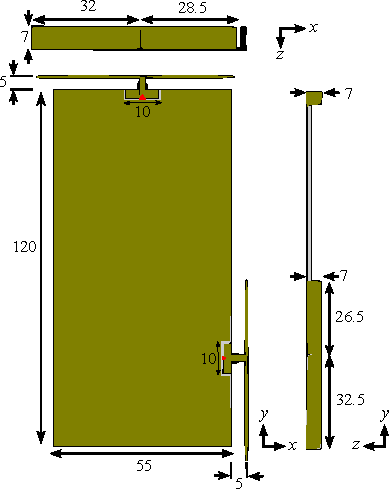
\includegraphics{img/tech_sol/monopole/5mm/3d_drawing/3d_drawing}
        \caption{Technical drawing. The ground clearance is here \SI{5}{mm}.}
        \label{fig:ant1technical_6pf}
    \end{subfigure}
    \hfill
    \begin{subfigure}[b]{0.49\linewidth}
        \centering
        \includegraphics{img/tech_sol/schematic_tuning_1}\\[1cm]
\footnotesize
        \begin{tabular}{|l|l|l|l|}
            \hline
            & $C_1$ & $L_1$ & $C_2$ \\
            \hline
            Top antenna & \SI{2.23}{pF} & \SI{3.94}{nH} & $[0.6,6]\,$pF\\
            Side antenna & \SI{2.15}{pF} & \SI{3,17}{nH} & $[1.2,12]\,$pF\\
            \hline
        \end{tabular}
        \caption{Tuning/matching circuit.}
        \label{fig:ant1_tuning}
    \end{subfigure}
    \caption{Technical drawing and tuning circuit for the antenna.  The matching circuit is applied for both the top and the side antenna.}
    \label{fig:ant1techschem_6pf}
\end{figure}

The $S_{11}$ and the efficiency, for different ground clearances, can be seen in Figure~\ref{fig:eff_s11_mono_sim_5mm}.
The simulation sweep is done from \SI{10}{mm} to \SI{3}{mm} ground clearance in \SI{1}{mm} steps and only for the top antenna. Each ground clearance simulation is matched and tuned independently to get the highest bandwidth possible in each case.

From the $S_{11}$ results, it is clear that the bandwidth decreases as the ground clearance decreases. The most noticeable results is at \SI{5}{mm} clearance as the bandwidth from this point does not increase significantly when increasing the ground clearance. However, decreasing the ground clearance further to \SI{4}{mm} and \SI{3}{mm}, the bandwidth drops significantly. Based on these results, it has been chosen to minimize the antenna design to a ground clearance of \SI{5}{mm}.

The efficiency ground clearance comparison shows similar results. In the high band, it is clear that decreasing the ground clearance will also decrease the bandwidth. However, the high band results are hard to compare as the different simulations are matched at different frequencies to gain the highest bandwidth. The comparison is more noticeable in the low band where it is clear that the lower the clearance, the lower the efficiency. Generally, the efficiency does not drop that much when decreasing the ground clearance. It should be possible to increase the efficiency by compensating for the drop using tunable capacitors.  

\begin{figure}[htbp]
   \begin{subfigure}[b]{0.49\linewidth}
        \centering
        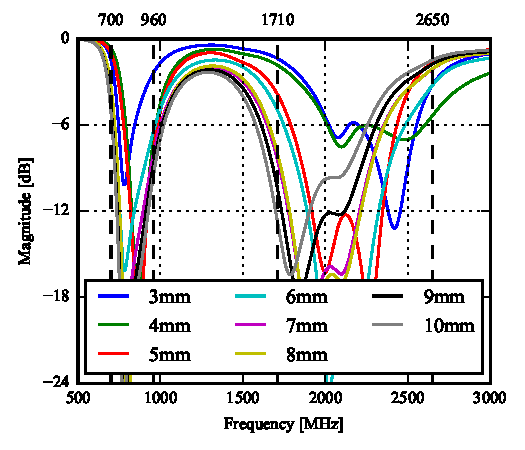
\includegraphics{img/tech_sol/monopole/5mm/s11_5mm}
        \caption{$S_{11}$ parameter for the top antenna, when sweeping the ground clearance.}
        \label{fig:s11_mono_sim_5mm}
    \end{subfigure}
    \hfill
    \begin{subfigure}[b]{0.49\linewidth}
        \centering
        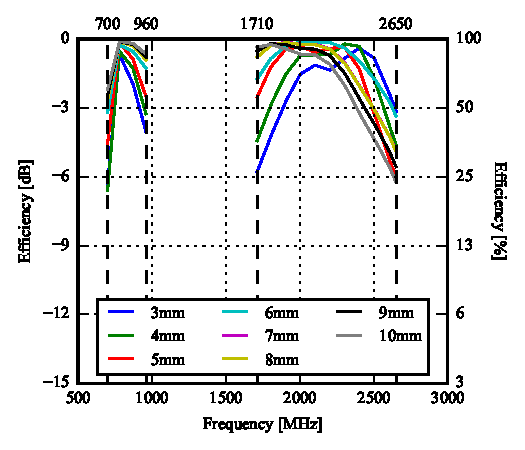
\includegraphics{img/tech_sol/monopole/5mm/eff_5mm}
        \caption{Efficiency for the top antenna, when sweeping the ground clearance.}
        \label{fig:eff_mono_sim_5mm}
    \end{subfigure}
    \caption{$S_{11}$ and efficiency for the top antenna, when sweeping the ground clearance from \SI{3}{mm} to \SI{10}{mm}}
    \label{fig:eff_s11_mono_sim_5mm}
\end{figure}

A sweep on the antenna height was also carried out from \SI{7}{mm} to \SI{4}{mm} with a ground clearance of \SI{5}{mm}. The results are not included as the top antenna was unable to cover the high band at anything lower than \SI{7}{mm}. To create a small-volume antenna it is therefore found that a trade-off between height and ground clearance must be made.

\FloatBarrier
\section{Simulation}

The simulated $S$-parameter sweep for both the top and the side antenna can be seen in Figure~\ref{fig:sparam_mono_6pf_free_space}. The bandwidth results can be seen in Table~\ref{tab:bw_sol1_6pf}. Both antennas fulfill the requirement for the low band, but in the high band, the top antenna experiences some problems. The top antenna lacks \SI{76}{MHz} of bandwidth in the high band. The lack of \SI{76}{MHz} bandwidth is acceptable as it covers close to the \SI{720}{MHz} requirement.
From the results, it is seen that both antennas cover the entire low band. In the high band, both the top and the bottom antenna experiences some problems at the band limits where the return loss decreases to \SI{5}{dB} and \SI{4}{dB}, respectively. The isolation has improved a bit compared to the results from the first design but is still significant in the lower band.     

The tuned efficiency for both antennas can be seen in Figure~\ref{fig:eff_sol1_6pf_free}. From the results, it is seen that both antennas are capable of covering the high band with an efficiency greater than \SI{-3}{dB}. In the low band, a lot of tuning is needed to achieve an efficiency around \SI{-3}{dB}. Generally, the efficiency drops as the capacity increases as expected.

%bandwidth table
\begin{table}
  \centering
  \begin{tabular}{|l|l|r|r|r|}
    \hline
    Antenna & Band & Start [MHz] & Stop [MHz] & Bandwidth [MHz] \\
    \hline
    Top     & Low  & 964         & 1128      & 164 \\
    Side    & Low  & 990         & 1118      & 128 \\
    \hline
    Top     & High & 1908        & 2574       & 666 \\
    Side    & High & 1829        & 2559      & 1270 \\
    \hline
  \end{tabular}
  \caption{Maximum bandwidth obtained in the low and high band for the top and the side antenna, respectively.}
  \label{tab:bw_sol1_6pf}
\end{table}

% Sweeping S-parameters
\begin{figure}[htbp]
   \begin{subfigure}[b]{0.49\linewidth}
        \centering
        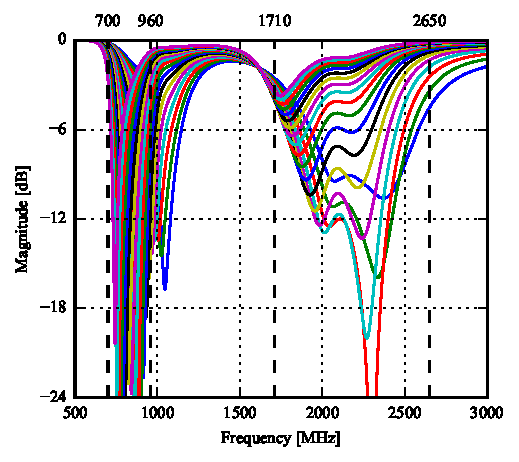
\includegraphics{img/tech_sol/monopole/5mm/sim/sweep_s11}
        \caption{$S_{11}$, sweeping $C_1$ and fixing $C_2$.}
    \end{subfigure}
    \hfill
    \begin{subfigure}[b]{0.49\linewidth}
        \centering
        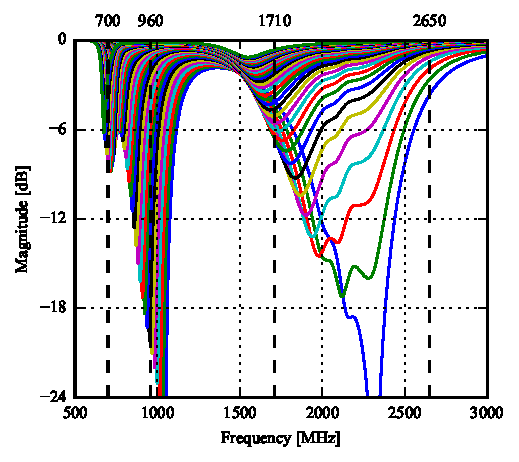
\includegraphics{img/tech_sol/monopole/5mm/sim/sweep_S22_12p}
        \caption{$S_{22}$, sweeping $C_2$ and fixing $C_1$.}
    \end{subfigure}
~
    \begin{subfigure}[b]{0.49\linewidth}
        \centering
        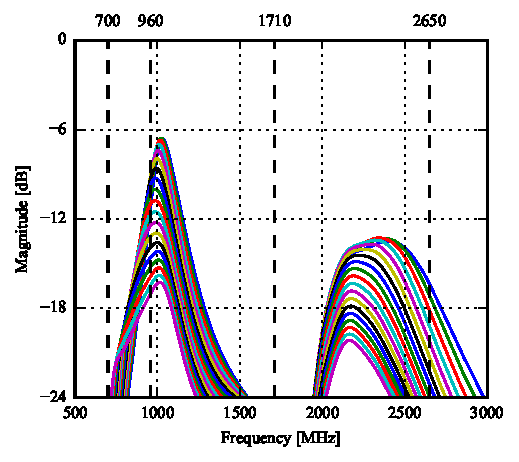
\includegraphics{img/tech_sol/monopole/5mm/sim/sweep_s11_s21}
        \caption{$S_{21}$, sweeping $C_1$ and fixing $C_2$.}
    \end{subfigure}
    \hfill
    \begin{subfigure}[b]{0.49\linewidth}
        \centering
        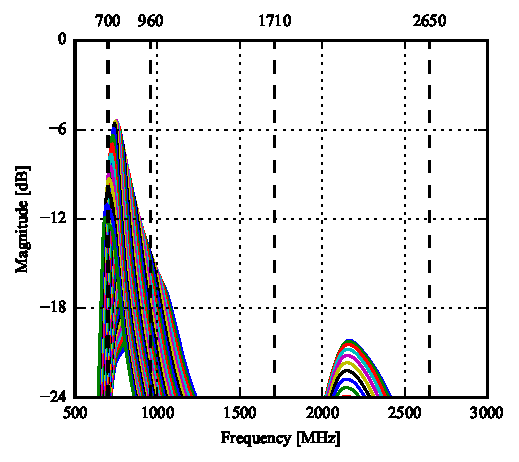
\includegraphics{img/tech_sol/monopole/5mm/sim/sweep_s22_s21_12p}
        \caption{$S_{21}$, sweeping $C_2$ and fixing $C_1$.}
    \end{subfigure}
    \caption{$S$-parameter sweep in free-space for tuning the shunt capacitor of each antenna, $C_1$ and $C_2$ for port 1 and 2, respectively. Port 1 is the top antenna and port 2 is the side antenna.}
    \label{fig:sparam_mono_6pf_free_space}
\end{figure}

% Sweeping Efficiency
\begin{figure}[htbp]
    \centering
    \begin{subfigure}{0.49\linewidth}
        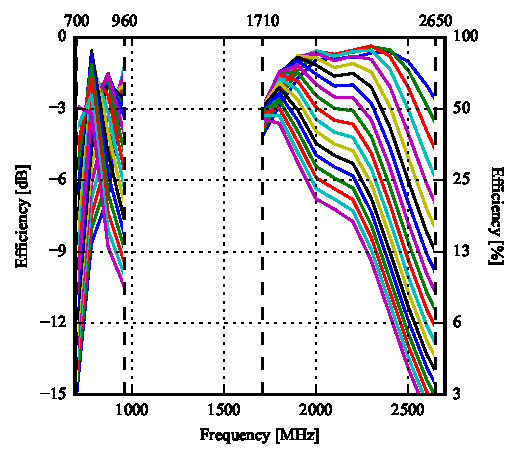
\includegraphics{img/tech_sol/monopole/5mm/6pf_eff_ac1}
        \caption{Sweeping $C_1$ and fixing $C_2$.}
    \end{subfigure}
    \hfill
    \begin{subfigure}{0.49\linewidth}
        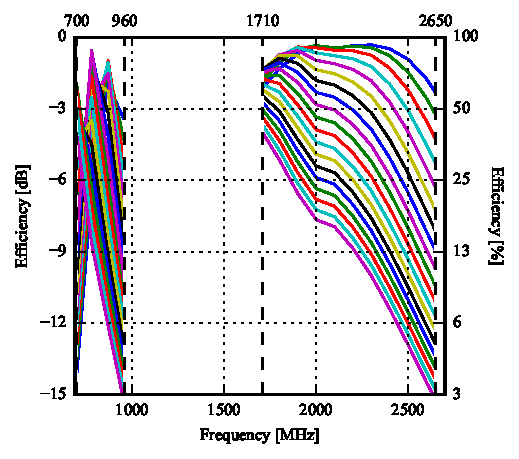
\includegraphics{img/tech_sol/monopole/5mm/6pf_eff_ac2}
        \caption{Sweeping $C_2$ and fixing $C_1$.}
    \end{subfigure}
    \caption{Efficiency for each antenna when sweeping the tunable capacitors. Here, $C_1$ and $C_2$ are the tuning capacitor for the top and side antenna, respectively.}
    \label{fig:eff_sol1_6pf_free}
\end{figure}

\FloatBarrier
\section{Measurements}
A comparison between the simulated and measured $S$-parameters and efficiencies can be seen in Figure~\ref{fig:mono_proto_sparam_eff5}. The component values used in the measurements can be seen in Table~\ref{fig:matching_mono_mini_meas}. From the $S$-parameters, it is seen that both antennas are detuned and have poor performance from \SI{2000}{MHz} to \SI{3000}{MHz}. The maximum bandwidth from the measurements can be seen in Table~\ref{tab:bw_mono_mini_meas}. Both antennas cover the bandwidth requirements in the low band but experiences some problems in the high band. The top antenna and the side antenna lack \SI{500}{MHz} and \SI{620}{MHz} bandwidth, respectively. 
The efficiency is also quite low as a result of the poor return loss of the high band.

\begin{figure}[htbp]
        \centering
        \begin{tabular}{m{3in}m{3in}}
            \centering
            \includegraphics{img/tech_sol/schematic_tuning_1}&
            \centering
            \footnotesize
            \begin{tabular}{|l|l|l|l|}
                \hline
                & $C_1$ & $L_1$ & $C_2$ \\
                \hline
              Top antenna & \SI{3.9}{pF} & \SI{1.6}{nH} & \SI{0.6}{pF} \\
                Side antenna & \SI{3}{pF} & \SI{1}{nH} & \SI{1.2}{pF} \\
                \hline
            \end{tabular}
        \end{tabular}
    \caption{Matching circuit for the minimized monopole prototype. These are the component values where the bandwidth is found to be the largest.}
    \label{fig:matching_mono_mini_meas}
\end{figure}

\begin{figure}[htbp]
    \centering
    \begin{subfigure}{0.49\linewidth}
        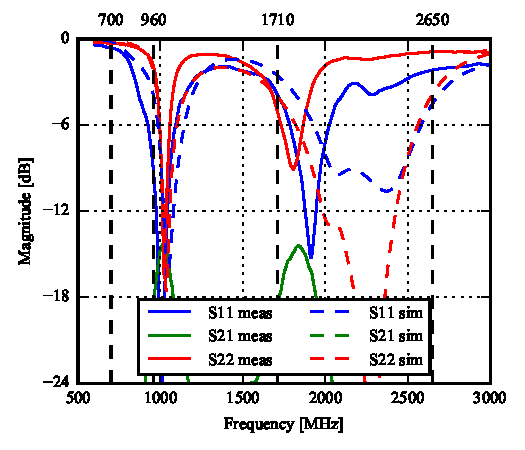
\includegraphics{img/tech_sol/monopole/5mm/sparams_comp.pdf}
        \caption{$S$-parameters.}
    \end{subfigure}
    \hfill
    \begin{subfigure}{0.49\linewidth}
        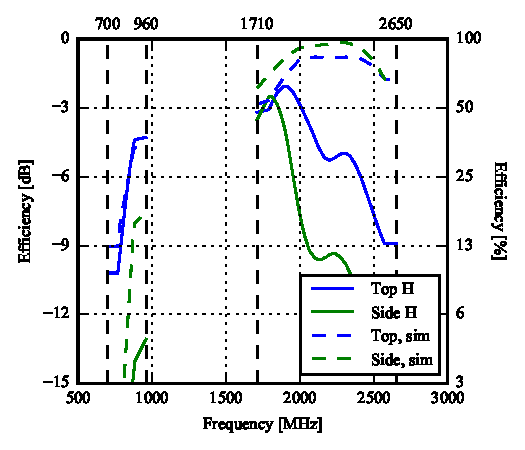
\includegraphics{img/tech_sol/monopole/5mm/eff_comp.pdf}
        \caption{Total efficiency.}
    \end{subfigure}
    \caption{$S$-parameters and total efficiency of the minimized monopole antenna prototype with the component values from Figure~\ref{fig:matching_mono_mini_meas}.}
    \label{fig:mono_proto_sparam_eff5}
\end{figure}

\begin{table}
  \centering
  \begin{tabular}{|l|l|r|r|r|}
    \hline
    Antenna & Band & Start [MHz] & Stop [MHz] & Bandwidth [MHz] \\
    \hline
    Top     & Low  & 920         & 1100       & 180 \\
    Side    & Low  & 1000        & 1080        & 80 \\
    \hline
    Top     & High & 1800        & 2020       & 220 \\
    Side    & High & 1710        & 1810       & 100 \\
    \hline
  \end{tabular}
  \caption{Maximum bandwidth obtained in the low and high band for the top and the side antenna, respectively.}
  \label{tab:bw_mono_mini_meas}
\end{table}

The $S$-parameter sweep for both the top and the side antenna can be seen in Figure~\ref{fig:sparam_mono_mini_meas}. From the $S_{11}$ and $S_{22}$ sweeps, it is seen that sweeping the capacitors does not improve the high band coverage. However, it is possible to cover the low band quite well but the high band needs some improvements for both antennas.  
The minimum isolation is measured in the low band at \SI{13}{dB}. 

The efficiency sweep is seen in Figure~\ref{fig:eff_mono_mini_meas}. The top antenna almost covers the entire low band with an efficiency of \SI{-6}{dB} but as expected, it experiences poor performance from \SI{2000}{MHz} to \SI{2650}{MHz}. The side antenna covers the low band with an efficiency going from \SI{-8.5}{dB} to \SI{-4.6}{dB} and has an efficiency above \SI{-6}{dB} from \SI{1710}{MHz} to \SI{1850}{MHz} where it drops below \SI{-9}{dB}.

\begin{figure}[htbp]
   \begin{subfigure}[b]{0.49\linewidth}
        \centering
        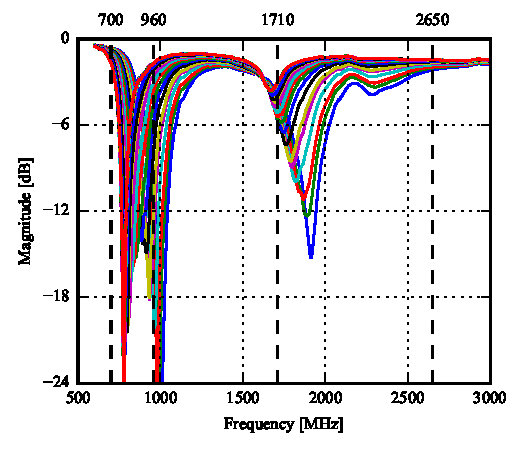
\includegraphics{img/tech_sol/monopole/5mm/meas/S11.pdf}
        \caption{$S_{11}$, sweeping $C_1$ and fixing $C_2$.}
    \end{subfigure}
    \hfill
    \begin{subfigure}[b]{0.49\linewidth}
        \centering
        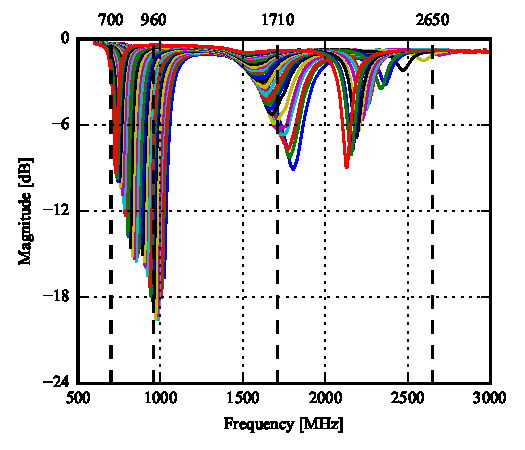
\includegraphics{img/tech_sol/monopole/5mm/meas/S22.pdf}
        \caption{$S_{22}$, sweeping $C_2$ and fixing $C_1$.}
    \end{subfigure}
~
\center
    \begin{subfigure}[b]{0.49\linewidth}
        \centering
        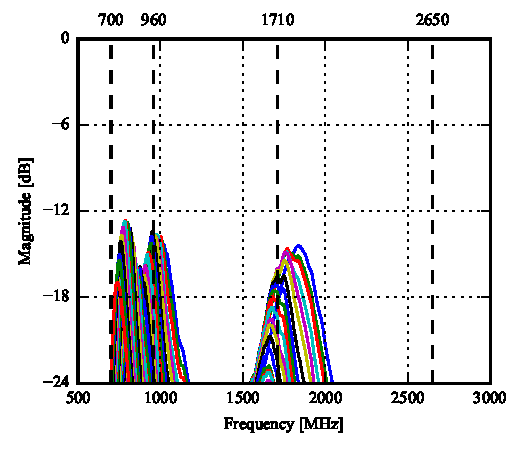
\includegraphics{img/tech_sol/monopole/5mm/meas/S21.pdf}
        \caption{$S_{21}$, sweeping $C_1$ and fixing $C_2$.}
    \end{subfigure}
    \caption{$S$-parameter sweep in free-space for tuning the shunt capacitor of each antenna, $C_1$ and $C_2$ for port 1 and 2, respectively. Port 1 is the top antenna and port 2 is the side antenna.}
    \label{fig:sparam_mono_mini_meas}
\end{figure}

\begin{figure}[htbp]
    \centering
    \begin{subfigure}{0.49\linewidth}
        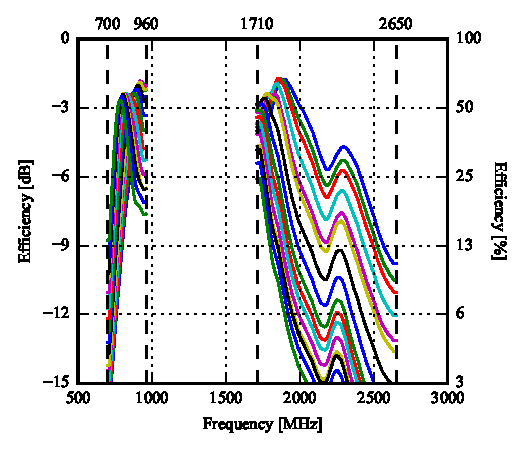
\includegraphics{img/tech_sol/monopole/5mm/meas/efficiency_top}
        \caption{Sweeping $C_1$ and fixing $C_2$.}
    \end{subfigure}
    \hfill
    \begin{subfigure}{0.49\linewidth}
        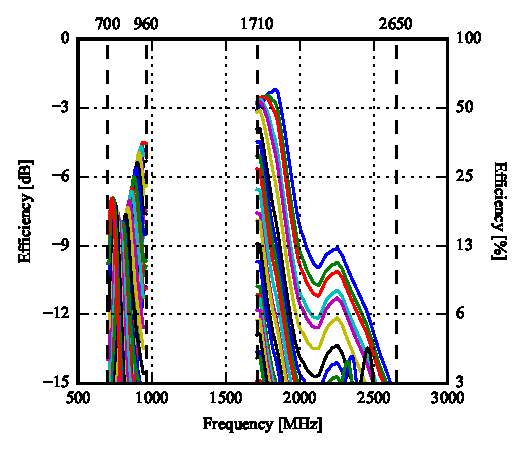
\includegraphics{img/tech_sol/monopole/5mm/meas/efficiency_side}
        \caption{Sweeping $C_2$ and fixing $C_1$.}
    \end{subfigure}
    \caption{Efficiency for each antenna when sweeping the tunable capacitors. Here, $C_1$ and $C_2$ are the tuning capacitor for the top and side antenna, respectively.}
    \label{fig:eff_mono_mini_meas}
\end{figure}


\section{Conclusion}
It is found, as expected, that a larger ground clearance makes it possible to get a larger bandwidth. However, it has been found that even with only \SI{5}{mm} ground clearance, a decent design can be made for a digitally tunable antenna.

A very simple antenna has been designed, simulated, and measured on a PCB with a MEMS tuner. It appears to be on a par with the preliminary design during the simulation phase. However, the measurement results showed a significant detuning and drop in efficiency and return loss when the PCB with MEMS tuner was used. Especially, the high band was hard to get resonating on the board. The design will therefore be modified to resonate better at high frequencies before it is used for the final measurements.

The next chapter will first describe the implementation of the triangle-feed antenna with the PCB and MEMS tuner as well. The design from this chapter will, at the same time, be revised to cover the high band better. The development, simulations, measurements, and refinements of this antenna will also be covered in the following.
